\chapter{Case Study}
\sisetup{per-mode=fraction}

\section{Data}
For the simulation a time horizon of one year is chosen. Of all available data the most recent ones were chosen.
Most of the data used for this thesis origins from SBB: the data for their existing hydro power plants, the corresponding natural inflow, the data for their frequency converters and the load profiles. The weather data for solar and wind was taken from MeteoSwiss \cite{idaweb}. 

\subsection{Load}
SBB provided the load profile from 2018. For the simulations of the year 2030, a prognosis based on this load profile was made by the experts of SBB. 

\subsection{Hydro Power}
\subsubsection{General Parameters for Hydro Power}
For this case study the density of water and the acceleration due to gravity were chosen as 
$\rho = \SI{1000}{\kg\per\cubic\metre}$ and $g = \SI{9.81}{\metre\per\square\second}$. According to the experts at SBB the efficiency of all hydro turbines and pumps were chosen as $\eta^{\text{t}} = \si{80}{\%}$ and $\eta^{\text{pump}} = \si{78}{\%}$ respectively. 

\subsubsection{Run of River Power Plants}
The set of run of river power plants $\textbf{R}$, their installed power $P^{\text{max}}_{r}$ and head $h_r$ are listed in Table~\ref{tab:sbb_ror}. The natural inflow data $Q^{\text{in,nat}}_{r, t}$ for each power plant $r$ was provided by SBB.  

\begin{table}[]
    \centering
    \begin{tabular}{|c|c|c|}
        \hline
         \textbf{Plant} & \textbf{Installed Power} & \textbf{Head} \\ \hline
         $r$ & $P^{\text{max}}_{r}$ & $h_r$ \\
         & [MW] & [m] \\\hline
            Göschenen            & 21.8 & 340    \\\hline
            Wassen~              & 29   & 277    \\\hline
            Amsteg~              & 120  & 280    \\\hline
            Massaboden           & 7.6  & 44     \\\hline
            Gösgen~              & 8    & 15.25   \\\hline
            Rupperswil-Auenstein & 20.9 & 10.675   \\\hline
            Trient~              & 0.7  & 130      \\\hline
            Vernayaz~            & 93   & 645      \\\hline
            Mühleberg            & 8    & 20     \\\hline 
    \end{tabular}
    \caption{Run of river power plants of SBB}
    \label{tab:sbb_ror}
\end{table}

\subsubsection{Hydro Dam Power Plants}
The set of hydro dam power plants $\textbf{D}$, their installed power $P^{\text{max}}_{d}$, head $h_d$, lower and upper volume boundaries $V^{\text{min}}_{d}$ and $V^{\text{max}}_{d}$ are listed in Table~\ref{tab:sbb_dam}. The inflow $Q^{\text{in,nat}}_{d,t}$ into each hydro dam power plant $d$ was provided by SBB. 

\begin{table}[]
    \centering
    \begin{tabular}{|c|c|c|c|c|}
        \hline
         \textbf{Plant} & \textbf{Installed Power} & \textbf{Head} & \textbf{Min. Volume} & \textbf{Max. Volume} \\
          $d$ & $P^{\text{max}}_{d}$ & $h_d$ & $V^{\text{min}}_{d}$ & $V^{\text{max}}_{d}$\\
          & [MW] & [m] & [$\si{\cubic\metre}$] & [$\si{\cubic\metre}$] \\\hline
            Göschenen   & 80 & 700 & 0 & 74’664’500 \\\hline
            Ritom       & 44 & 850 & 0 & 48’550’000   \\\hline
    \end{tabular}
    \caption{Hydro dam power plants of SBB}
    \label{tab:sbb_dam}
\end{table}

According to historical data from SBB the initial lake level at the beginning of the year was chosen to be $70\% \cdot V^{\text{max}}_{d}$. 

\subsubsection{Hydro Pumped Storage Power Plants}
The set of hydro pump power plants $\textbf{P}$, their installed discharge power $P^{\text{dis,max}}_{p}$, charge power $P^{\text{cha,max}}_{p}$, head $h_p$ and volume boundaries $V^{\text{min}}_{d}$ and $V^{\text{max}}_{d}$ are listed in Table~\ref{tab:sbb_pump}. The natural inflow data $Q^{\text{in,nat}}_{p,t}$ into each hydro dam power plant $p$ was given by SBB. 

\begin{table}[h!]
    \centering
    \begin{tabular}{|C{2cm}|C{2cm}|C{2cm}|C{1cm}|C{2cm}|C{2cm}|}
        \hline
         \textbf{Plant} & \textbf{Discharge Power} & \textbf{Charge Power} & \textbf{Head} & \textbf{Min. Volume} & \textbf{Max. Volume} \\
          $r$ & $P^{\text{dis,max}}_{p}$ & $P^{\text{cha,max}}_{p}$ & $h_p$ & $V^{\text{min}}_{p}$ & $V^{\text{max}}_{p}$\\
          & [MW] & [MW] & [m] & [$\si{\cubic\metre}$] & [$\si{\cubic\metre}$] \\\hline
            Chatelard  & 106.9 & 30 & 807.5 & 0 & 224’604’000 \\\hline
            Etzelwerk       & 125 & 57 & 480 & 0 & 91’957’000   \\\hline
    \end{tabular}
    \caption{Hydro pump power plants of SBB}
    \label{tab:sbb_pump}
\end{table}

According to historical data from SBB the initial lake level at the beginning of the year was chosen to be $70\% \cdot V^{\text{max}}_{p}$. 

\subsection{Exchange with 50Hz Grid}
\subsubsection{Frequency Converters}
The frequency converters $f$ of SBB and their maximum import power $P^{\text{imp,max}}_{f}$ and export power $P^{\text{exp,max}}_{f}$ are listed in Table~\ref{tab:sbb_freqtrans}. 

\begin{table}[h!]
    \centering
    \begin{tabular}{|c|c|c|}
        \hline
         \textbf{Transformer} & \textbf{Import Power} & \textbf{Export Power} \\ \hline
         $f$ & $P^{\text{imp,max}}_{f}$ & $P^{\text{exp,max}}_{f}$ \\
         & [MW] & [MW] \\\hline
        Giubiasco 1     & 26.5  & 25    \\\hline
        Kerzers 12      & 71.6  & 67.5    \\\hline
        Massaboden1     & 30    & 32   \\\hline
        Rupperswil12    & 59    & 53.2     \\\hline
        Seebach12       & 126.2 & 120  \\\hline
        Wimmis uf2      & 26.5  & 25   \\\hline
        Giubiasco23     & 40    & 42   \\\hline
        Wimmis1245      & 80    & 80   \\\hline
        Obermatt1       & 3     & 3      \\\hline
        Winkeln12       & 112   & 108      \\\hline
 
    \end{tabular}
    \caption{Frequency converters of SBB}
    \label{tab:sbb_freqtrans}
\end{table}

\subsubsection{Cost of Exchange}
The spot price was taken from a Hourly Price Forward Curve (HPFC) for 2019 of SBB. For 2019 the 'Kostendeckende Einspeisevergütung' (cost-covering feed-in tariff) $KEV$ is 23\,CHF/MW \cite{KEV}, the 'Arbeitstarif' (working tariff for grid usage) $AT$ is  1.9\,CHF/MW and the 'Systemdienstleistungen' (system service tariff) $SDL$ is 3.8\,CHF/MW (composed of 2.4\,CHF/MW of general ancillary services tariff and 1.4\,CHF/MW of individual ancillary services tariff) \cite{tariff}. 

\subsection{Solar Power}\label{chap:data solar}
\subsubsection{General Parameters}
In agreement with the experts of SBB a solar panel efficiency of $\eta^\text{s} = \SI{20}{\percent}$ was used. 

\subsubsection{Global Radiation}
The global radiation data was taken from Meteoswiss \cite{idaweb}. To find a weather representative data set for Switzerland the data platform proposes a data package of 24 weather representative locations (see Fig.~\ref{fig:24Locations}). For simplicity reasons the mean of the global radiation of this 24 locations was taken. 
For the scenarios assuming that solar panels will only be distributed in the alpine regions, only the global radiation data of Adelboden, Davos, Disentis, Samedan and Zermatt was taken and averaged. All this data was measured in 2018.

\begin{figure}
    \centering
    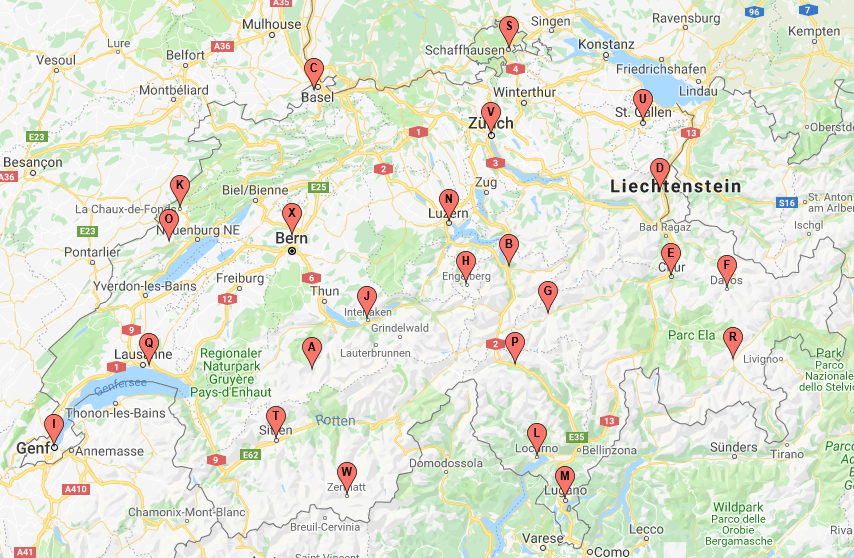
\includegraphics[width = \textwidth]{figures/24_Locations.jpg}
    \caption{24 weather representative locations in Switzerland \cite{batchgeo}. Legend:\newline A:	Adelboden, B: Altdorf, C: Binningen, D: Buchs, E: Chur, F: Davos, G: Disentis, H: Engelberg, I: Genf, J: Interlaken, K: La Chaux-de-Fonds, L: Locarno, M: Lugano, N: Luzern, O: Neuenburg, P: Piotta, Q: Pully, R: Samedan, S: Schaffhausen, T: Sitten, U: St. Gallen, V: Zürich, W: Zermatt, X: Zollikofen}
    \label{fig:24Locations}
\end{figure}

\subsection{Wind Power}
\subsubsection{General Parameters}
The roughness length $z_0$ is chosen to be $\SI{0.2}{\m}$. According to \cite{windspeed} this corresponds to a roughness length for agricultural terrain with many houses, bushes and plants or $\SI{8}{\m}$ high hedges in the surrounding of $\SI{250}{\m}$. 

\subsubsection{Wind Speed}
The wind speed data was taken from Meteoswiss \cite{idaweb}. As mentioned in Chapter~\ref{chap:data solar} the platform proposes 24 weather representative locations for Switzerland. The data was measured in 2018 and is available in averages of 10\,min granularity. It is assumed, that this measurement was taken at $\SI{1}{\metre}$ height. 

\subsubsection{Wind Turbine}
As wind turbine type the "Windkraft Zürcher 300\,kW" was chosen. Its parameters can be seen in Table~\ref{tab:wind_turbine_zurcher}. In discussion with the experts of SBB this choice was made due to the following reasons: This turbine is a newly developed horizontal turbine of relatively small dimensions compared to other turbine models. According to the producer, turbines of this type can by placed in close proximity to buildings and to each other. This allows for a higher power density in terms of turbines per $\SI{}{\square\metre}$. Furthermore, due to the small dimensions of one turbine, the opposition of residents in the proximity might be less vehement than with big horizontal wind turbines. 


\begin{table}[h!]
\centering
\begin{tabular}{|l|c|} \hline
    \textbf{Parameter} & \\ \hline
     Rated Power & $\SI{300}{\kW}$ \\ \hline
     Hub Height & $\SI{22}{\m}$  \\ \hline
     Cut in Wind Speed & $\SI{1.2}{\meter\per\second}$ \\ \hline
     Rated Wind Speed & $\SI{10}{\meter\per\second}$ \\ \hline
     Cut out Wind Speed & $\SI{30}{\meter\per\second}$ \\ \hline
\end{tabular}
\caption{Parameters of the Windkraft Zürcher 300\,kW turbine taken from \cite{zurcher}}
\label{tab:wind_turbine_zurcher}
\end{table}


\section{Results}
In this section the results of the scenarios are presented. First, the motivation for each scenario is explained. Afterwards the dependency on the weighting factors is elaborated. Finally the results in terms of renewable generation units are presented. 

\subsection{Motivation for Different Scenarios}
For this case study several scenarios were simulated. A list of the scenarios can be found in Table~\ref{tab:scenarios}. 

Scenarios 1-3 were simulated without any share of renewables. The purpose of this was to get an impression of how close to reality the simulations get and how to tune the weighting factor. 

Scenarios 4-6 were simulated with a share of renewables of 10\%, while the model was free to chose how much solar and how much wind should be invested. Furthermore, these three scenarios enabled again to check the tuning of the weighting factors. 

In scenarios 7-9 a share of renewables of 10\% was given. Given this condition the model was forced to use a defined share of solar or wind, i.e. either 50\% of both or either only solar or only wind. Scenario 7 and 8, which have a forced share of solar, were made due to the fact, that investments in solar are more practicable in Switzerland than investments in wind. Nevertheless, scenario 9 had to check how much capacity in wind would be needed, if this was the only renewable source. 

A share of renewables of 20\% was considered in scenarios 10-13. The motivation behind this scenarios is the evolution of the granting of the water concessions. Again the model was free to chose between solar and wind in scenario 10, while it was forced to a certain share of solar and a certain share of wind in scenarios 11-13. 

In scenarios 14 and 15 the model only considered global radiation from alpine regions in Switzerland. The reason for this scenarios is the assumption, that especially during winter months there is much more radiation in the alpine regions than in the rest of Switzerland. This could be a promising solution since the load of SBB is higher during winter due to heating of trains and the hydro generation is missing during this time. The share of renewables was however forced to 10\%. The alpine regions were chosen to be: Adelboden, Davos, Disentis, Samedan and Zermatt. Scenario 14 enabled to see what share in solar and wind the model proposes itself, while scenario 15 was done to compare the solar investment with scenario 7, where the only change in parameters is the location of solar. 

Finally, a future load profile of the year 2030 was considered in scenarios 16 and 17. It has to be mentioned, that no other parameters were changed, i.e. the cost factors and weather data remained unchanged neglecting yearly changes. The share of renewables was set to 10\%. Scenario 16 enabled to see what share in solar and wind the model proposed itself, while scenario 17 was done to compare the investment with scenario 7, where the only change in parameters is the load profile.  

\begin{table}[h!]
\centering
\begin{tabular}{|C{1.5cm}|C{1.5cm}|C{2cm}|C{2cm}|C{2cm}|C{2cm}|} \hline
    \textbf{Scenario} 
    & \textbf{Load Profile} 
    & \textbf{Location of Solar} 
    & \textbf{Weighting of Cost}
    & \textbf{Share of Renewables}
    & \textbf{Share of Solar and Wind} \\ \hline
    1   & 2018  & Switzerland & 1       & 0\%    & free\\ \hline
    2   & 2018  & Switzerland & $10^{20}$ & 0\%    & free\\ \hline
    3   & 2018  & Switzerland & $10^{-20}$ & 0\%    & free\\ \hline
    4   & 2018  & Switzerland & 1       & 10\%    & free\\ \hline
    5   & 2018  & Switzerland & $10^{20}$ & 10\%    & free\\ \hline
    6   & 2018  & Switzerland & $10^{-20}$ & 10\%    & free\\ \hline
    7   & 2018  & Switzerland & $10^{-20}$ & 10\%    & 50\% / 50\% \\ \hline
    8   & 2018  & Switzerland & $10^{-20}$ & 10\%    & 100\% / 0\% \\ \hline
    9   & 2018  & Switzerland & $10^{-20}$ & 10\%    & 0\% / 100\% \\ \hline
    10  & 2018  & Switzerland & $10^{-20}$ & 20\%    & free\\ \hline
    11  & 2018  & Switzerland & $10^{-20}$ & 20\%    & 50\% / 50\% \\ \hline
    12  & 2018  & Switzerland & $10^{-20}$ & 20\%    & 100\% / 0\% \\ \hline
    13  & 2018  & Switzerland & $10^{-20}$ & 20\%    & 0\% / 100\% \\ \hline
    14  & 2018  & Alps        & $10^{-20}$ & 10\%    & free \\ \hline
    15  & 2018  & Alps        & $10^{-20}$ & 10\%    & 50\% / 50\%  \\ \hline
    16  & 2030  & Switzerland & $10^{-20}$ & 10\%    & free \\ \hline
    17  & 2030  & Switzerland & $10^{-20}$ & 10\%    & 50\% / 50\%  \\ \hline
    
\end{tabular}
\caption{Simulated Scenarios}
\label{tab:scenarios}
\end{table}

The results of each scenario and its energy dispatch can be found in the appendix. 

\subsection{Dependency on Weighting Factors}\label{chapter_weighting factor}
A key element of the model are the weighting factors in the objective function~\eqref{objective function}. To estimate the effect of the weighting factors, simulations to all extremes were made for the cases with no renewables (scenarios 1-3) and with a 10\% share in renewables (scenario 4-6). In scenario 1 and 4, all weighting factors were set equal to one. In scenarios 2 and 5, the weighting factor for exchange cost was set to $W_3 = 10^{20}$, giving the cost a very high weight compared to the curtailments. Finally, in scenarios 3 and 6, the weighting factor for exchange cost was set to $W_3 = 10^{-20}$, giving the cost a very low importance compared to the curtailments. In Fig.~\ref{fig:results scenario 1-6} the power dispatch of scenarios 1-6 are shown. 

For scenarios 1-3, where no solar and wind are considered, one can observe the following: since there are no renewable energies, the curtailment in all three scenarios are always equal to zero. Therefore the only remaining element in the objective function is the cost of the exchange. Therefore all three scenarios should show in the exact same result, regardless of the weighting factors. However, one can see that scenario 3 has a different result. It is assumed that this happens due to numerical issues, since a weighting factor of $10^-20$ is very small. 

Over all the import power peaks are observed to be much higher than in reality. This might be due to the fact, that in reality it is never the case that all frequency converters are fully available due to maintenance or renovation work. 

On the other side the energy distribution of all this three scenarios is the same: approximately 75\% of the energy is produced by hydro power plants while the remaining quarter is provided by the exchange (See Fig.~\ref{fig:result_water_levels} right). According to the experts of SBB this corresponds to reality.

However, the water levels do not fully correspond to the real operation pattern (See Fig.~\ref{fig:result_water_levels} left). In reality, all lake levels follow an almost sinusoidal pattern, being empty in May and filled up again by the beginning of October. While the patterns of the results follow approximately this pattern there are several deviations: The water levels of the dam power plant lakes Göschenen and Ritom show the most realistic pattern. Just during the months March - May the lakes are empty while in reality they should be only empty in May. 

The lake of the pumped power plant Etzelwerk shows a different pattern: while it is emptied until March, it afterwards gets filled up again to stay above a certain level during the months June til October. This is due to the mosquito level which is defined as a constraint for this lake only and therefore corresponds to reality. 

Finally the lake of pumped power plant Chatelard has the biggest deviations: first of all there is an almost instant water level change at the first of October. This is due to the fact, that at the first of October this power plant gets access to an additional small lake (Lac du Vieux Emosson). This is represented by a large inflow corresponding to the level of that additional lake at one time step. Furthermore, the lake does never get empty. This is due to the fact, that the inflow into the lake is very low, which is not enough to fill up the lake from empty in May until full in October. 

\begin{figure}
    \centering
    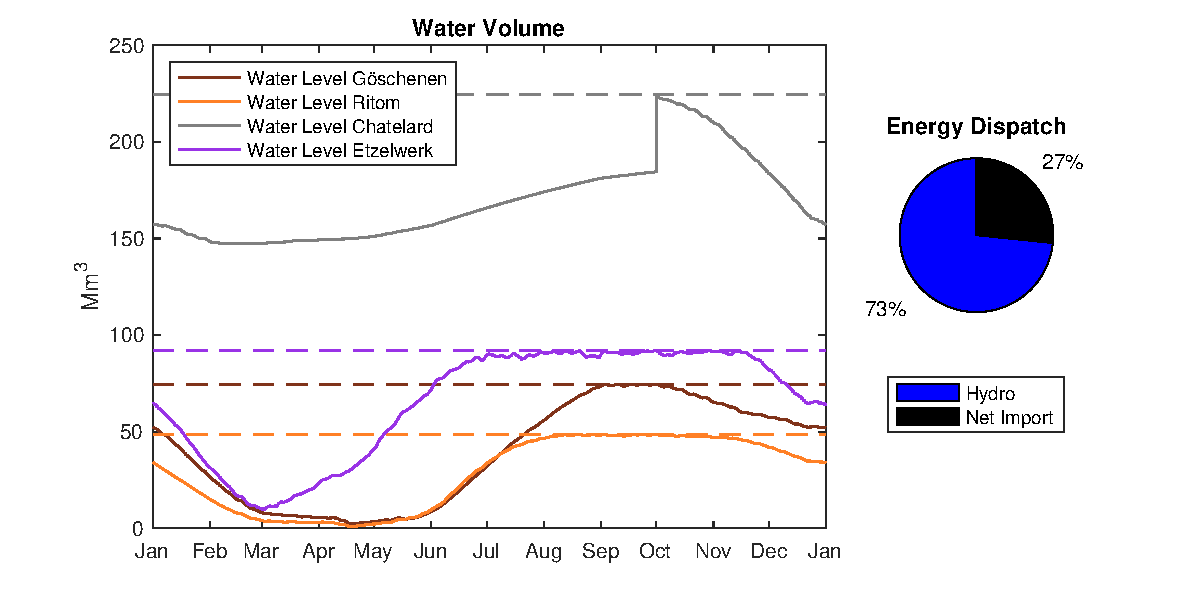
\includegraphics[width=\textwidth]{figures/Results/waterlevel_and_energydispatch_scenario1.pdf}
    \caption{Water levels of individual lakes and energy dispatch of Scenario 1.}
    \label{fig:result_water_levels}
\end{figure}

Lets hoewever consider the scenarios 4-6, where a share of solar and wind of 10\%  is introduced. One can observe the following: 

If all weighting factors are equal to one (i.e. scenario 4), the cost of the exchange gets a very high importance. This is due to the fact, that the cost is in the range of $10^7$. The model proposes to install 231\,MW in wind. This way a huge amount of energy can be exported when prices are very high. The reason why the model only invests in wind and not in solar is, that wind power is available when the prices are high, i.e. in winter and in the morning and evening. Solar power is rarely available in these periods. However, since the energy of wind and solar is limited to exactly 10\% of the total consumed energy, this also means that the curtailment is in the range of $10^7$, because no wind is used during the other periods. 

In scenario 5 the weighting factor of exchange cost is set to $W_3 = 10^{20}$. As a result, the effect described above is enforced: The model invests more in wind (4794\,MW) than in scenario 4 to be able to bring the cost down even more by exporting huge amounts of  energy when prices are high. This huge investment is enabled since no investment cost are considered.

Finally, in scenario 6 the weighting factor of exchange cost is set to $W_3 = 10^{-20}$. Now the cost has a very low order of magnitude in the objective function, and therefore it loses importance compared to the curtailment of wind and solar. The model proposes a investment of 52\,MW in wind and 1\,MW in solar. This choice was made due to the following reasons: solar energy is available during lunchtime and is much more intense in summer then in winter. However the load profile of SBB is high during in the morning and afternoon due to rush hour traffic and it is higher in winter than in summer due to the heating of the trains. Therefore the model prioritizes wind energy, since this is available also during peak load and high price times. The investment of 1\,MW in solar is a result of the strict equality constraint for the renewable target (see constraint~\eqref{const:renewable}). With 173 turbines only 9.95\% of the total consumed energy can be produced. Therefore, the model fills the remaining 0.05\% gap with 1\,MW of solar instead of investing in 174 turbines, since this would lead to a big curtailment. 

Since scenario 6 corresponds the most to reality, this set of weighting factors (i.e. $W_1 = W_2 = 1$ and $W_3 = 10^{-20}$) will be used for all following simulations. However, any different weighting factor might lead to different results. 

\begin{figure}
    \centering
    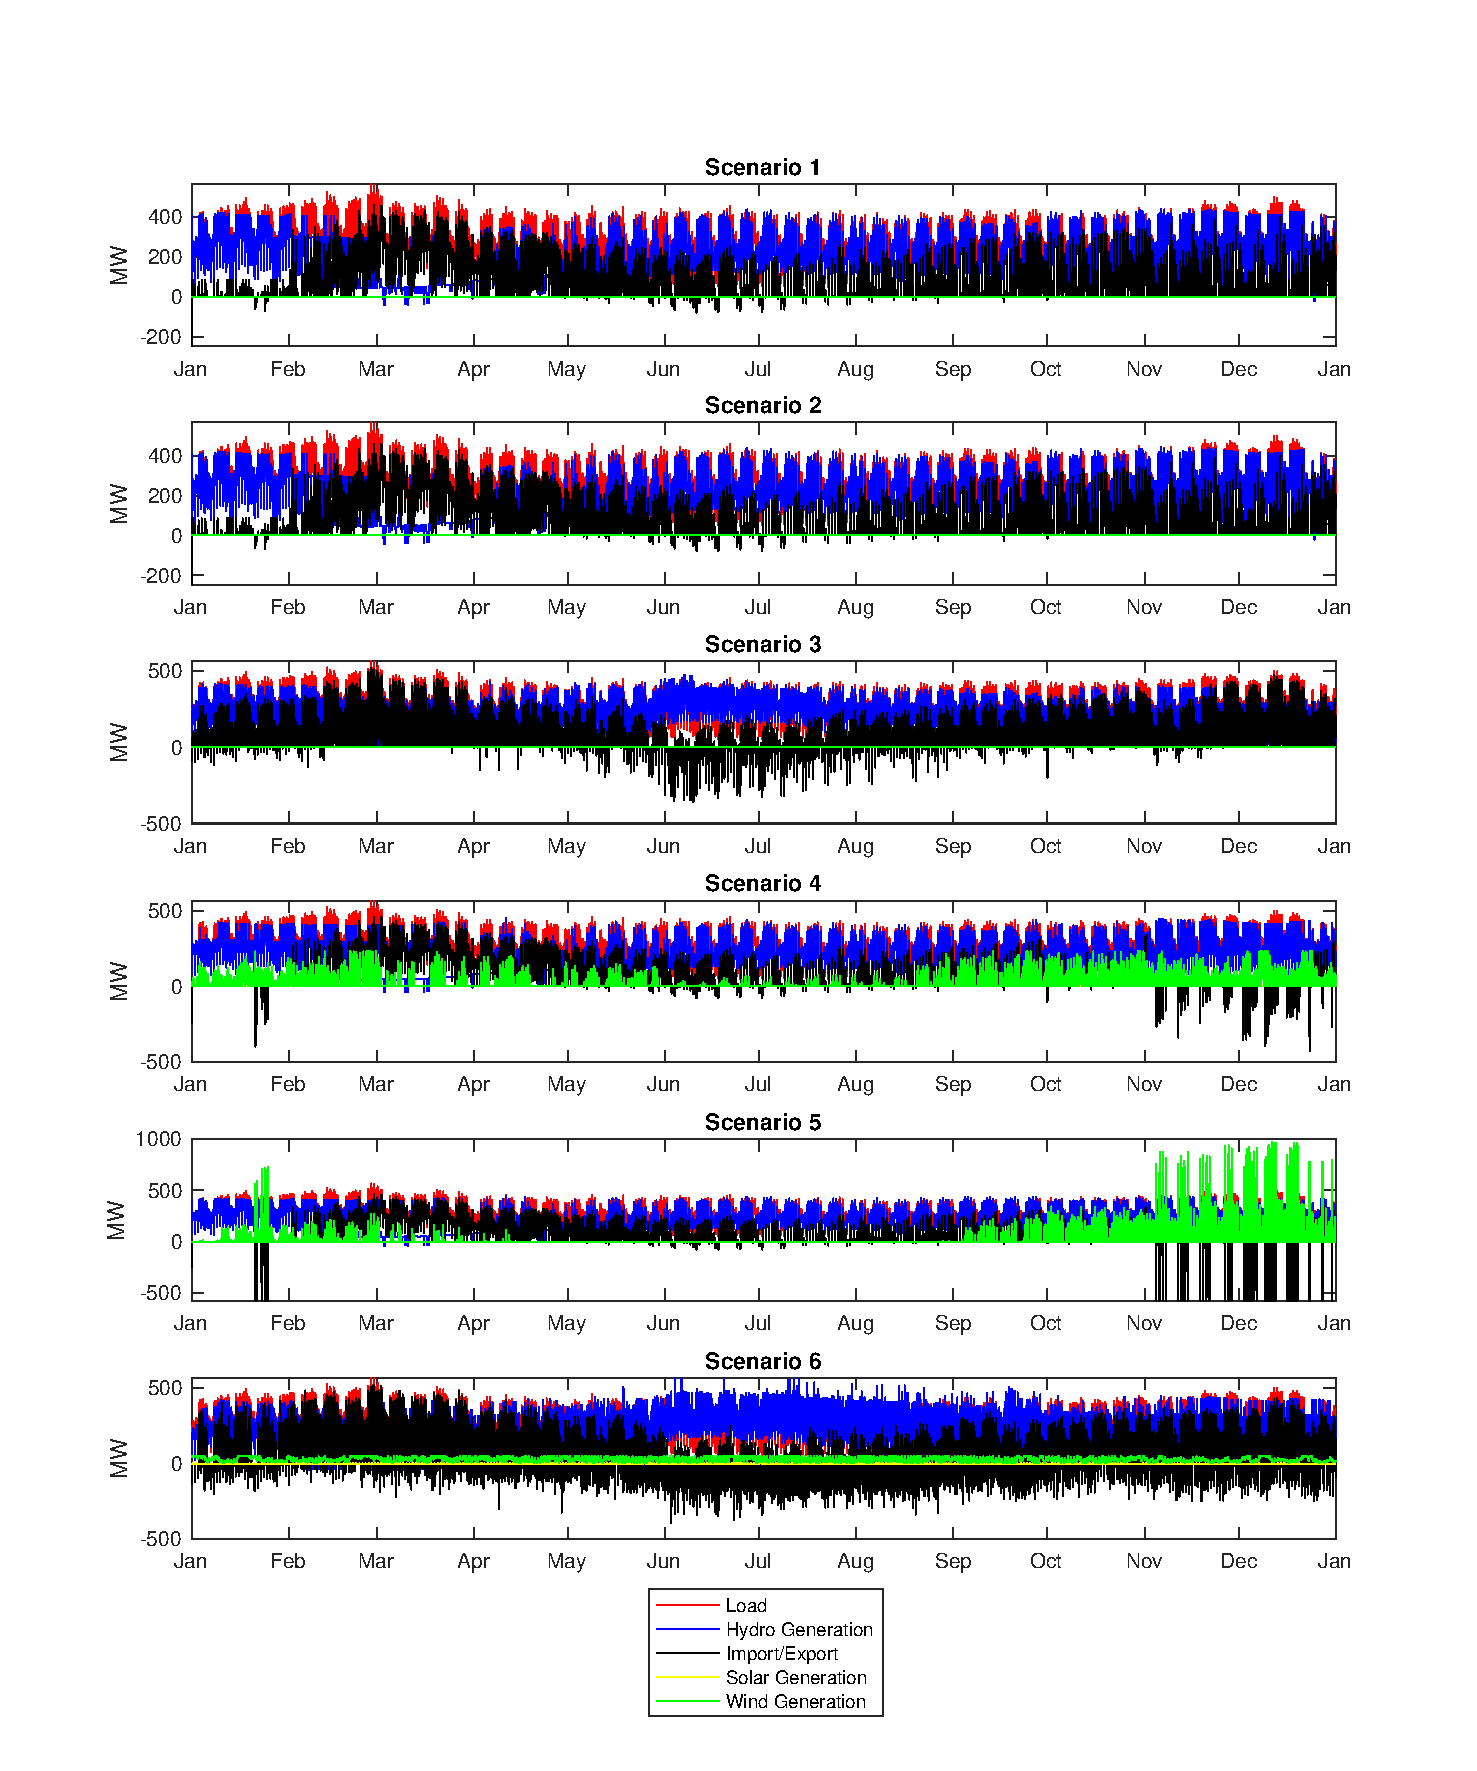
\includegraphics[width=\textwidth]{figures/Results/power_dispatch_scenario_123456.pdf}
    \caption{Power dispatch over one year for scenarios 1-6. Scenarios 1-3 are without renewables while scenarios 4-6 are with a 10\% share of renewables. Weighing factors: \\
    Scenario 1 \& 4: $W_1 = W_2 = 1$ and $W_3 = 1$, \\
    Scenario 2 \& 5: $W_1 = W_2 = 1$ and $W_3 = 10^{20}$, \\
    Scenario 3 \& 6: $W_1 = W_2 = 1$ and $W_3 = 10^{-20}$.}
    \label{fig:results scenario 1-6}
\end{figure}

\subsection{Results of Scenarios}
All results of scenarios can be find in the appendix. 

Scenarios 1-6 were discussed in the Chapter~\ref{chapter_weighting factor}. 

Scenario 7 shows a 5\% share in solar and a 5\% share in wind. It therefore purposes to invest 89\,MW in solar and 26\,MW in wind (i.e. 87 turbines à 300\,kW). The resulting effect of the renewables on the daily power dispatch is small (see Fig.~\ref{fig:results days scenario 7}). While wind power is available almost permanently during the day as a kind of baseload, solar decreases the hydro generation slightly during the day. However, hydro generation and the exchange remain the main forces.

\begin{figure}
    \centering
    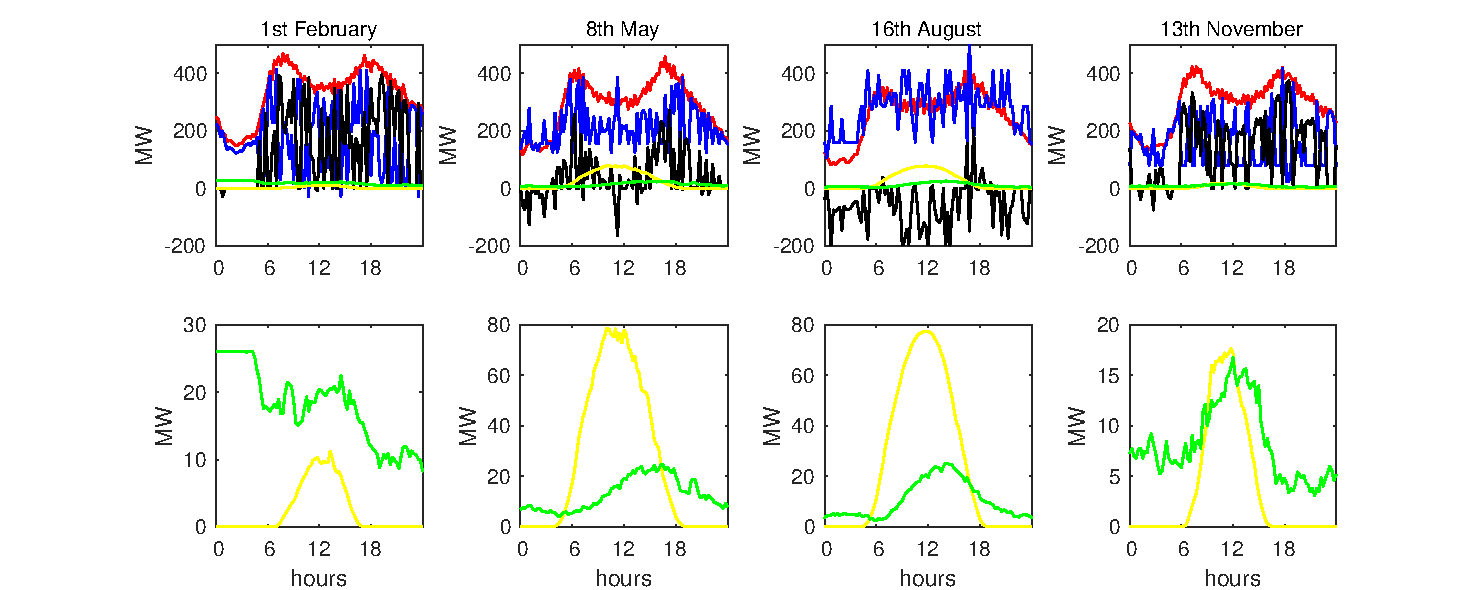
\includegraphics[width=\textwidth]{figures/Results/power_dispatch_days_scenario7.pdf}
    \caption{Power dispatch on four days during the year of scenario 7.}
    \label{fig:results days scenario 7}
\end{figure}

If only solar is considered as a 10\% share of renewables (scenario 8) the investment purposed is 177\,MW. On the other hand in scenario 9, if 10\% of wind is invested, the model gives an investment of 52\,MW (i.e. 174 turbines à 300\,kW).

Scenarios 10-13 consider a 20\% share of renewables. As in scenario 6, the model prioritizes wind over solar whenever it has free choice (scenario 10). It proposes and investment of 104\,MW in wind (i.e. 347 turbines à 300\,kW). In addition an investment of 1\,MW in solar is made, again due to the strict equality constraint as in scenario 6. 

Scenarios 11-13 have forced shares in solar or wind. Scenario 11 (10\% solar and 10\% wind) leads to an investment of 177\,MW in solar and 52\,MW in wind. If only solar is considered in scenario 12, an investment of 355\,MW is required. If wind is the only renewable source in the 20\% share, 104\,MW (i.e. 348 turbines à 300\,kW) are needed. 

In scenarios 14 and 15 the location of solar is limited to the alpine regions of Switzerland. If the model is free to chose the kind of renewable (scenario 14), it invests 50\,MW in wind and 6\,MW in solar. This solar investment produces 0.3\% of the total consumed energy. Even though this is a small part, this solar investment cannot be explained by the strict equality constraint anymore. The reason for this is the global radiation in the alpine regions: summing up all global radiation over one year, there is 5\% more radiation in the alps than in the mean over Switzerland. Considering only the winter months December, January and February the sum of all global radiation is even 30\% higher than in the mean over all Switzerland. Therefore, the model chooses itself a small share of solar. 

In scenario 15, where the model is forced to a 5\% share in each solar and wind, one can see that the investment in solar is 84\,MW. This is a reduction in investment of approximately 5\% compared to scenario 7, while both scenarios reach a 5\% share in solar energy. 

In scenarios 16 and 17 a future load profile was chosen. This load profile has increased peaks compared to the load profile in 2018 and the total energy consumption is 9\% higher. If the model is free to chose between wind and solar, it proposes and investment of 45\,MW in solar and 44\, in wind (i.e. 145 turbines à 300\,kW). This leads to a solar energy share of 2\% and 8\% of wind energy. The reason for this increased share in solar compared to the previous simulations is the increased load profile: since the load profile is increased in general, the energy demand over lunchtimes rises as well. This increased demand can be covered by solar energy. 

Scenario 17 finally shows, what investments are required if the percentages of wind and solar are fixed to 5\% each: 97\,MW in solar and 29\,MW in wind (i.e. 95 turbines à 300\,kW). 

